\chapter{Marco teórico.}

\mynote{Este capítulo sirve como una breve introducción a todos los métodos, conceptos y modelos considerados para el desarrollo de este trabajo.}

Todo proceso de clasificación de imágenes puede dividirse en los siguientes pasos:

\begin{itemize}
	\item Tratado inicial de las imágenes
	\item Extracción de características
	\item Tratamiento de datos
	\item Entrenamiento de modelo de clasificación
	\item Evaluación modelo de clasificación
\end{itemize}

\section{Extracción de características}
\label{section:Extracción de catacterísticas}

En este paso el objetivo es obtener información cuantitativa (númerica) de las muestras a partir de diversos métodos.\\ Por ejemplo, de una clasificación de números escritos a mano se pueden obtener características como el número de trazos, anchura del contorno, color, etc. Es decir, se obtienen una serie de propiedades informativas de la muestra para, después, entrenar el modelo de clasificación. 

Para este trabajo, se han utilizado los siguientes métodos:
\begin{itemize}
	\item Descriptores de Fourier
	\item Momentos de imagen (Momentos Hu)
	\item Descriptores locales binarios (\textit{Local Binary Patterns})
	\item Histograma de gradientes
	\item *Método propio
\end{itemize}

\subsection{Momentos de imagen.}

Los momentos de imagen son un promedio de las intensidades de una imagen binaria. La convención habitual define un momento \(M\) para una imagen binaria \(B\) de la siguiente forma:

\begin{equation}
	\label{eqn:momento}
	M_{ij} = \sum_{x}^{} \sum_{y}^{} x^{i} y^{j} B(x,y)
\end{equation}

Utilizando la ecuación \ref{eqn:momento}, se pueden obtener características la imagen como los centroides:
\begin{equation}
	\label{eqn:momentos_x_centroide}
	\overline{x} = \dfrac{M_{10}}{M_{00}}
\end{equation}
\begin{equation}
	\label{eqn:momentos_y_centroide}
	\overline{y} = \dfrac{M_{01}}{M_{00}}
\end{equation}

Sin embargo, aplicando una transformación a la ecuación \ref{eqn:momento}, se pueden obtener momentos invariantes a la traslación:

\begin{equation}
	\label{eqn:momentos_central}
	\mu_{i,j} = \sum_{x} \sum_{y} (x-\overline{x})^{i} (y-\overline{y})^{j} I(x,y)
\end{equation}

A la ecuación \ref{eqn:momentos_central} se la conoce como \textbf{momentos centrales}.

Además, aplicando otra transformación se pueden obtener momentos invariantes al escalado también:

\begin{equation}
	\label{eqn:momento_normalizado}
	\eta_{i,j} = \dfrac{\mu_{i,j}}{\mu_{00}^{\dfrac{i+j}{2}+1}}
\end{equation}

La fórmula \ref{eqn:momento_normalizado} se conoce como \textbf{momento centralizado}.

\subsubsection{Momentos de Hu}

Los momentos de Hu \cite{1057692} son un un conjunto de siete fórmulas obtenidas a partir de los momentos centralizados que permiten obtener siete momentos invariantes tanto a traslación, rotación, escalado y volteado (el séptimo momento es el invariante a volteado, cambiando de signo cuando la imagen es reflejada).


\begin{equation}
	\label{eqn:hu_momentos}
	\begin{split}
		M_{1} = \eta_{20} + \eta_{02} \\
		M_{2} = (\eta_{20}-\eta_{02})^{2} + 4\eta_{11}^{2} \\
		M_{3} = (\eta_{30}-3\eta_{12})^{2} + (3\eta_{21}-\eta_{03})^{2} \\
		M_{4} = (\eta_{30}+\eta_{12})^{2} + (\eta_{21}+\eta_{03})^{2} \\
		M_{5} & = (\eta_{30}-3\eta_{12})(\eta_{30}+\eta_{12})[(\eta_{30}+\eta_{12})^{2}-3(\eta_{21}+3\eta_{03})^{2}] \\
		& +(3\eta_{21}-\eta_{03})(\eta_{21}+\eta_{03})[3(\eta_{30}+\eta_{12})^{2}-(\eta_{21}+\eta_{03})^{2}] \\
		M_{6} & = (\eta_{20}-\eta_{02}[(\eta_{30}+\eta_{12})^{2}-(\eta_{21}+\eta_{03})^{2}] \\
		& +4\eta_{11}(\eta_{30}+\eta_{12})(\eta_{21}+\eta_{03}) \\
		M_{7} = (3\eta_{21}-\eta_{03})(\eta_{30}+\eta_{12})[(\eta_{30}+\eta_{12})^{2}-3(\eta_{21}+3\eta_{03})^{2}] \\
		& -(\eta_{30}-3\eta_{12})(\eta_{21}+\eta_{03})[3(\eta_{30}+\eta_{12})^{2}-(\eta_{21}+\eta_{03})^{2}]
	\end{split}
\end{equation}

A partir de \ref{eqn:hu_momentos}, se pueden obtener siete características númericas.

\pagebreak
\subsection{Histograma de gradientes}

El histograma de gradientes \cite{osti_6007283} es una técnica de extración de características muy utilizada en la detección de objetos.

A partir de una imagen binaria de dimensiones $ nxm $, se calculan los gradientes de intensidad, así como la magnitud y el ángulo:

\begin{equation}
	\label{eqn:hog_GxGy}
	\begin{split}		
		G_{x} = B(x+1,y) - B(x,y) \\
		G_{y} = B(x,y+1) - B(x,y)
	\end{split}
\end{equation}

La ecuación \ref{eqn:hog_GxGy} determina los gradientes de la imagen binaria \(B\). Tanto \(G_{x}\) como \(G_{y}\) son dos imágenes binarias con la información de gradientes en ejes X e Y, respectivamente. 
A partir de la ecuación \ref{eqn:hog_GxGy}, se obtienen las magnitudes y ángulos:

\begin{equation}
	\label{eqn:hog_mag}
	Mag_{(x,y)} (\mu)= \sqrt{G_{x}^{2}+G_{y}^{2}}
\end{equation}

\begin{equation}
	\label{eqn:hog_angulo}
	Ang_{(x,y)} (\theta) = \lvert tan^{-1}(\dfrac{G_{y}}{G_{x}})\lvert
\end{equation}

Tanto la ecuación \ref{eqn:hog_mag} como \ref{eqn:hog_angulo} representan imágenes binarias.

El siguiente paso consiste en dividir las imágenes de magnitud y ángulos en $ N $ cuadrículas, pudiendo ser $ N = 1 $ (una única cuadrícula).

Para cada cuadrícula se representa un histograma de 9 posiciones, con cada posición en el rango $ [\theta,\theta+\delta\theta) $. Convencionalmente, se suele utilizar $\delta\theta = 20^{\circ}$ . De esta forma se obtiene el siguiente histograma $ H_{N}$:

\begin{table}[htb]
	\centering
	\caption{Histograma de gradientes, tabla ejemplo}
	\label{tab:hog_histograma_tabla}
	\begin{tabular}{|c||c|c|c|c|c|c|c|c|c|}
		\hline
		Magnitud &    &    &    &    &    &     &     &     &     \\ \hline
		Ángulo   & 0  & 20 & 40 & 60 & 80 & 100 & 120 & 140 & 160 \\ \hline
	\end{tabular}
\end{table}

A cada intervalo angular y de magnitud, se le denomina $ \theta_{j} $ y $ \mu_{j} $, respectivamente, para $ j\:\epsilon\:[0,8]$ .

De tal forma, si en la cuadrícula $ N_{i} $ existe un $\theta_{x,y}$ que pertenece al rango $ [\theta,\theta+\delta\theta j) $, para $ j\:\epsilon\:[0,8]$, se determina que $ \mu_{j} = \mu_{x,y} + \mu_{j}$.

\begin{equation}
	\label{eqn:hog_sum_magnitudes}
	\mu_{j} = \sum{\mu_{x,y}} \iff \theta_{x,y}\:\epsilon\:[\theta,\theta+\delta\theta \cdot j)
\end{equation}

Existen casos en los que $\theta_{x,y} > 160^{\circ}$, entonces $\mu_{x,y}$ contribuye tanto a $ 0^{\circ} $ como a $160^{\circ}$.

\begin{equation}
	\setlength{\jot}{14pt}
	\label{eqn:hog_angulo_mayor_de_160}
	\begin{split}
		\dfrac{180-\theta_{x,y}}{20}\cdot \mu_{x,y}\:\implies\: [160,180) \\
		\left(1-\dfrac{180-\theta_{x,y}}{20}\right)\cdot \mu_{x,y}\:\implies\: [0,20)
	\end{split}	
\end{equation}

El último paso consiste en normalizar el histograma:

\begin{equation}
	\label{eqn:hog_histograma_normalizacion}
	\mu_{j} = \dfrac{\mu_{j}}{max\:(\mu_{j})}
\end{equation}

Tras la aplicación de \ref{eqn:hog_histograma_normalizacion}, se tienen $ 9\cdot N$ características, siendo $ N $ el número de cuadrículas.

\pagebreak
\subsection{Patrones locales binarios}

También conocido por sus siglas del inglés \textbf{LBP} (del inglés, \textit{Local Binary Patterns}), este método propuesto en la decada de 1990 \cite{572934} permite extraer un histograma de 256 características de una muestra.

\begin{figure}[H]
	\centering
	\captionsetup{justification=centering}
	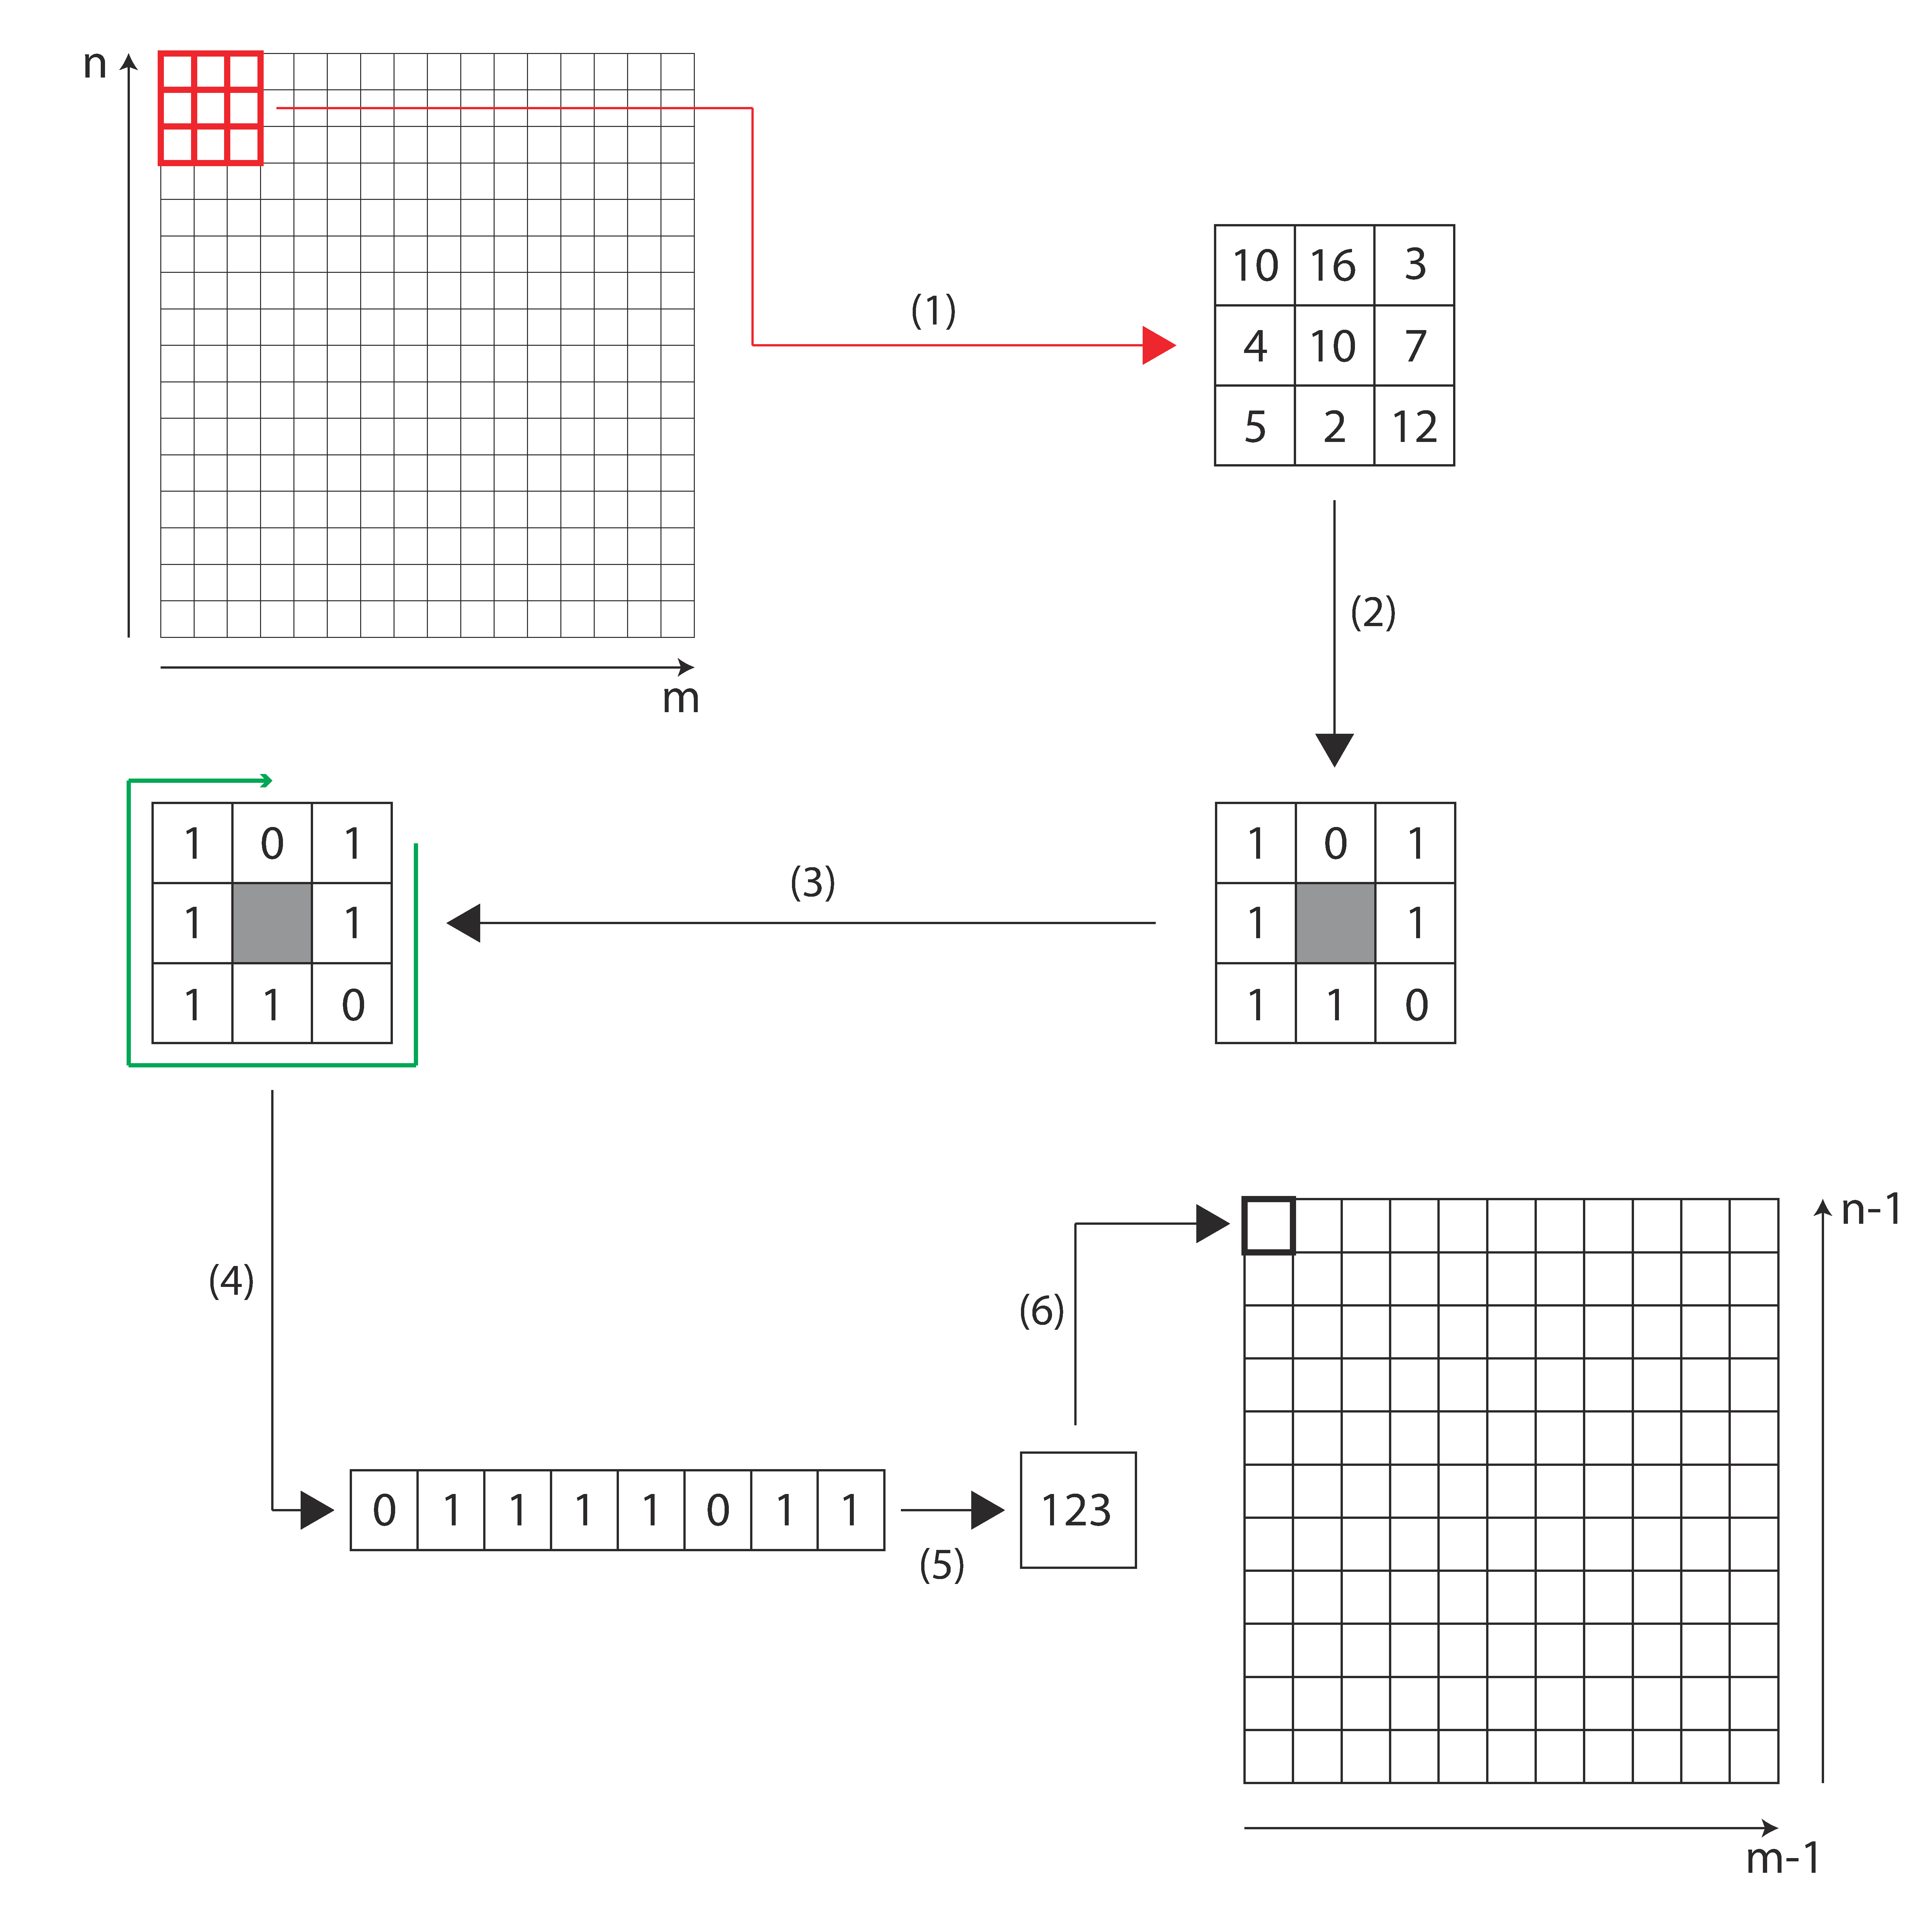
\includegraphics[width=\textwidth]{imagenes/marco_teorico/LBP/LBP_diagrama.pdf}
	\caption{Esquema método LBP}	
	\label{fig:LBP_diagrama}
\end{figure}

La figura \ref{fig:LBP_diagrama} muestra un esquematizado resumen del proceso de extración de características por este método.

La imagen original es tratada como una matriz de dimensiones $ n(filas) x\: m(columnas) $. A partir de esta, se extraen submatrices de dimensiones $3x3$ y se comienza el análisis de datos.

En la nueva submatriz, la posición central es comparada con las exteriores. Si, para una posición exterior, el valor central es menor o igual, se asigna a esta posición un valor 1. De ser mayor, se asigna un 0.

La nueva matriz binaria es tratada como un número binario de 8 dígitos, consisitiendo el siguiente paso en obtener el equivalente en base diez. Este último valor es almacenado en una nueva matriz de dimensiones $(n-1)x(m-1)$.

Realizando este proceso para toda la imagen original se tiene un conjunto de datos a partir de los cuales obtener el histograma sobre el que se basa el método \textbf{LBP}.

Teóricamente, el número máximo de características extraibles es 256 (ver \ref{eqn:LBP_rango}), pero pueden agruparse por rangos obteniendo grupos de características. Esta última opción es dependiente de la aplicación y del problema a tratar.

\begin{equation}
	[00000000, 11111111]_{2} \rightarrow [0, 255]_{10}
	\label{eqn:LBP_rango}
\end{equation}

\pagebreak
\subsection{Descriptores de Fourier}

Los descriptores de Fourier son un método de extracción de características por el cual un objeto bidimensional, cuyos puntos tienen las coordenadas $ (x_{k},\:y_{k})$, es mapeado a un dominio complejo de la forma $(x_{k},\:iy_{k})$. De tal forma, el objeto es tratado como una señal discreta compleja a la cual se aplica la transformada discreta de Fourier para encontrar sus armónicos (descriptores de Fourier).

La figura \ref{fig:fourier_poligono_trazo_continuo} representa una forma hexagonal rellena. Para obtener los descriptores de Fourier de este objeto, es necesario obtener el contorno exterior de la figura (véase \ref{fig:fourier_poligono_trazo_discontinuo}).

\begin{figure}[H]
	\centering
	\captionsetup{justification=centering}
	\begin{subfigure}{0.5\textwidth}
		\centering
		\captionsetup{justification=centering}
		
\includegraphics[width=0.5\textwidth]{imagenes/marco_teorico/Descriptores_Fourier/Poligono_trazo_continuo.pdf}	
		\caption{}
		\label{fig:fourier_poligono_trazo_continuo}
	\end{subfigure}
	\hfill
	\begin{subfigure}{0.7\textwidth}
		\centering
		\captionsetup{justification=centering}
		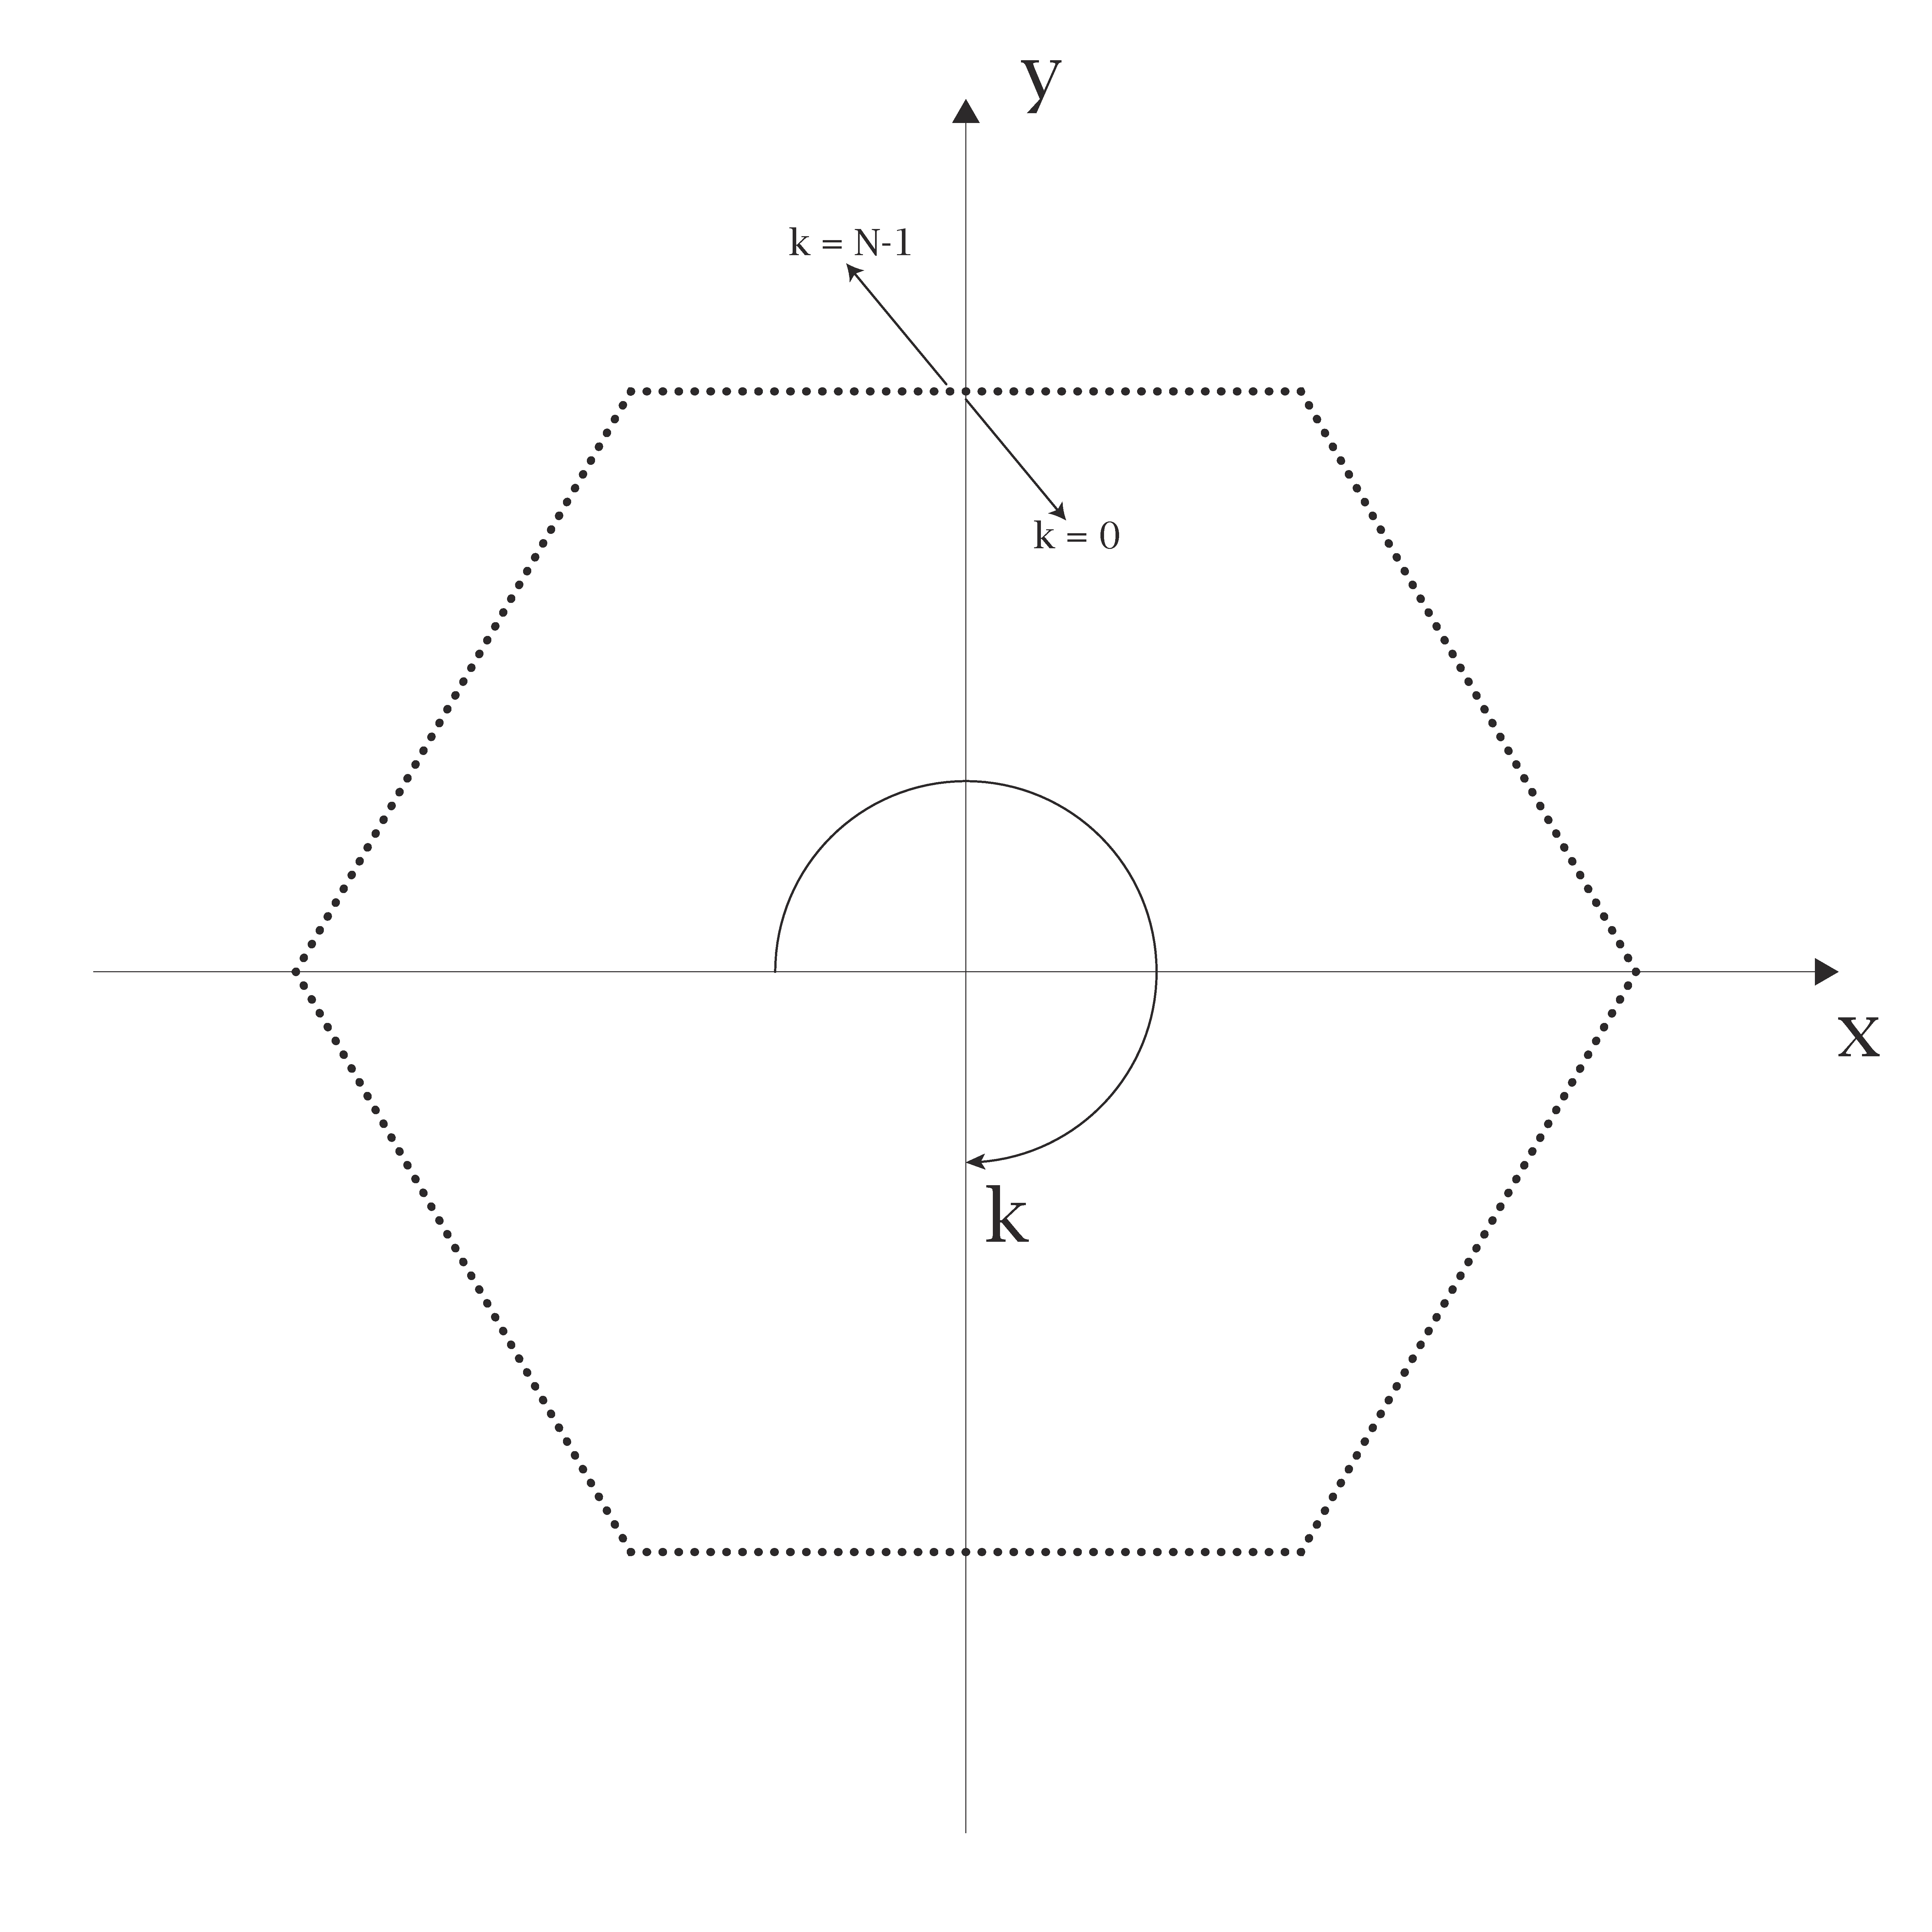
\includegraphics[width=0.7\textwidth]{imagenes/marco_teorico/Descriptores_Fourier/Poligono_ejesXY_k_figura.pdf}	
		\caption{}
		\label{fig:fourier_poligono_trazo_discontinuo}
	\end{subfigure}	
	\caption{Descriptores de Fourier}
	\label{fig:fourier_esquema}
\end{figure}

Este nuevo contorno está representado por $N$ puntos, de tal forma que cada punto puede definirse de la forma $ (x_{k},\:y_{k}),\:con\:k = 0, 1, 2, ..., N-1 $ y el contorno, a su vez, como la señal $f_{k} = (x_{k},\:y_{k})$.

Si $f_{k}$ es transformada al dominio complejo de la forma $f_{k} = x_{k} + iy_{k}$, es posible aplicar la transformada discreta de Fourier a $f_{k}$ para obtener los $N$ armónicos de la señal (descriptores de Fourier): 

\begin{equation}
	F_{m} = \sum_{k=0}^{N-1} f_{k}\cdot e^{-\dfrac{2\pi i}{N}mk},\qquad m = 0, 1, 2, ..., N-1
	\label{eqn:dft}
\end{equation}

La ecuación \ref{eqn:dft} (transformada discreta de Fourier), proporciona la serie de valores $ F_{0}, F_{1}, F_{2}, ..., F_{N-1} $, a partir de los cuales se obtienen los descriptores de Fourier (valores absolutos) $\lvert F_{0}, F_{1}, F_{2}, ..., F_{N-1} \rvert$.

En función de la resolución de la imagen original y su definición, el número de puntos del contorno $N$ variará, obteniéndose una cantidad diferente para cada caso. Por ello, el número de descriptores de Fourier obtenibles de cada imagen no será el mismo. Es por esto que, generalmente, de los $N$ descriptores obtenidos para cada imagen, se escogen solo $n\:|\:0\leq n\leq N$.

\begin{figure}[H]
	\centering
	\captionsetup{justification=centering}
	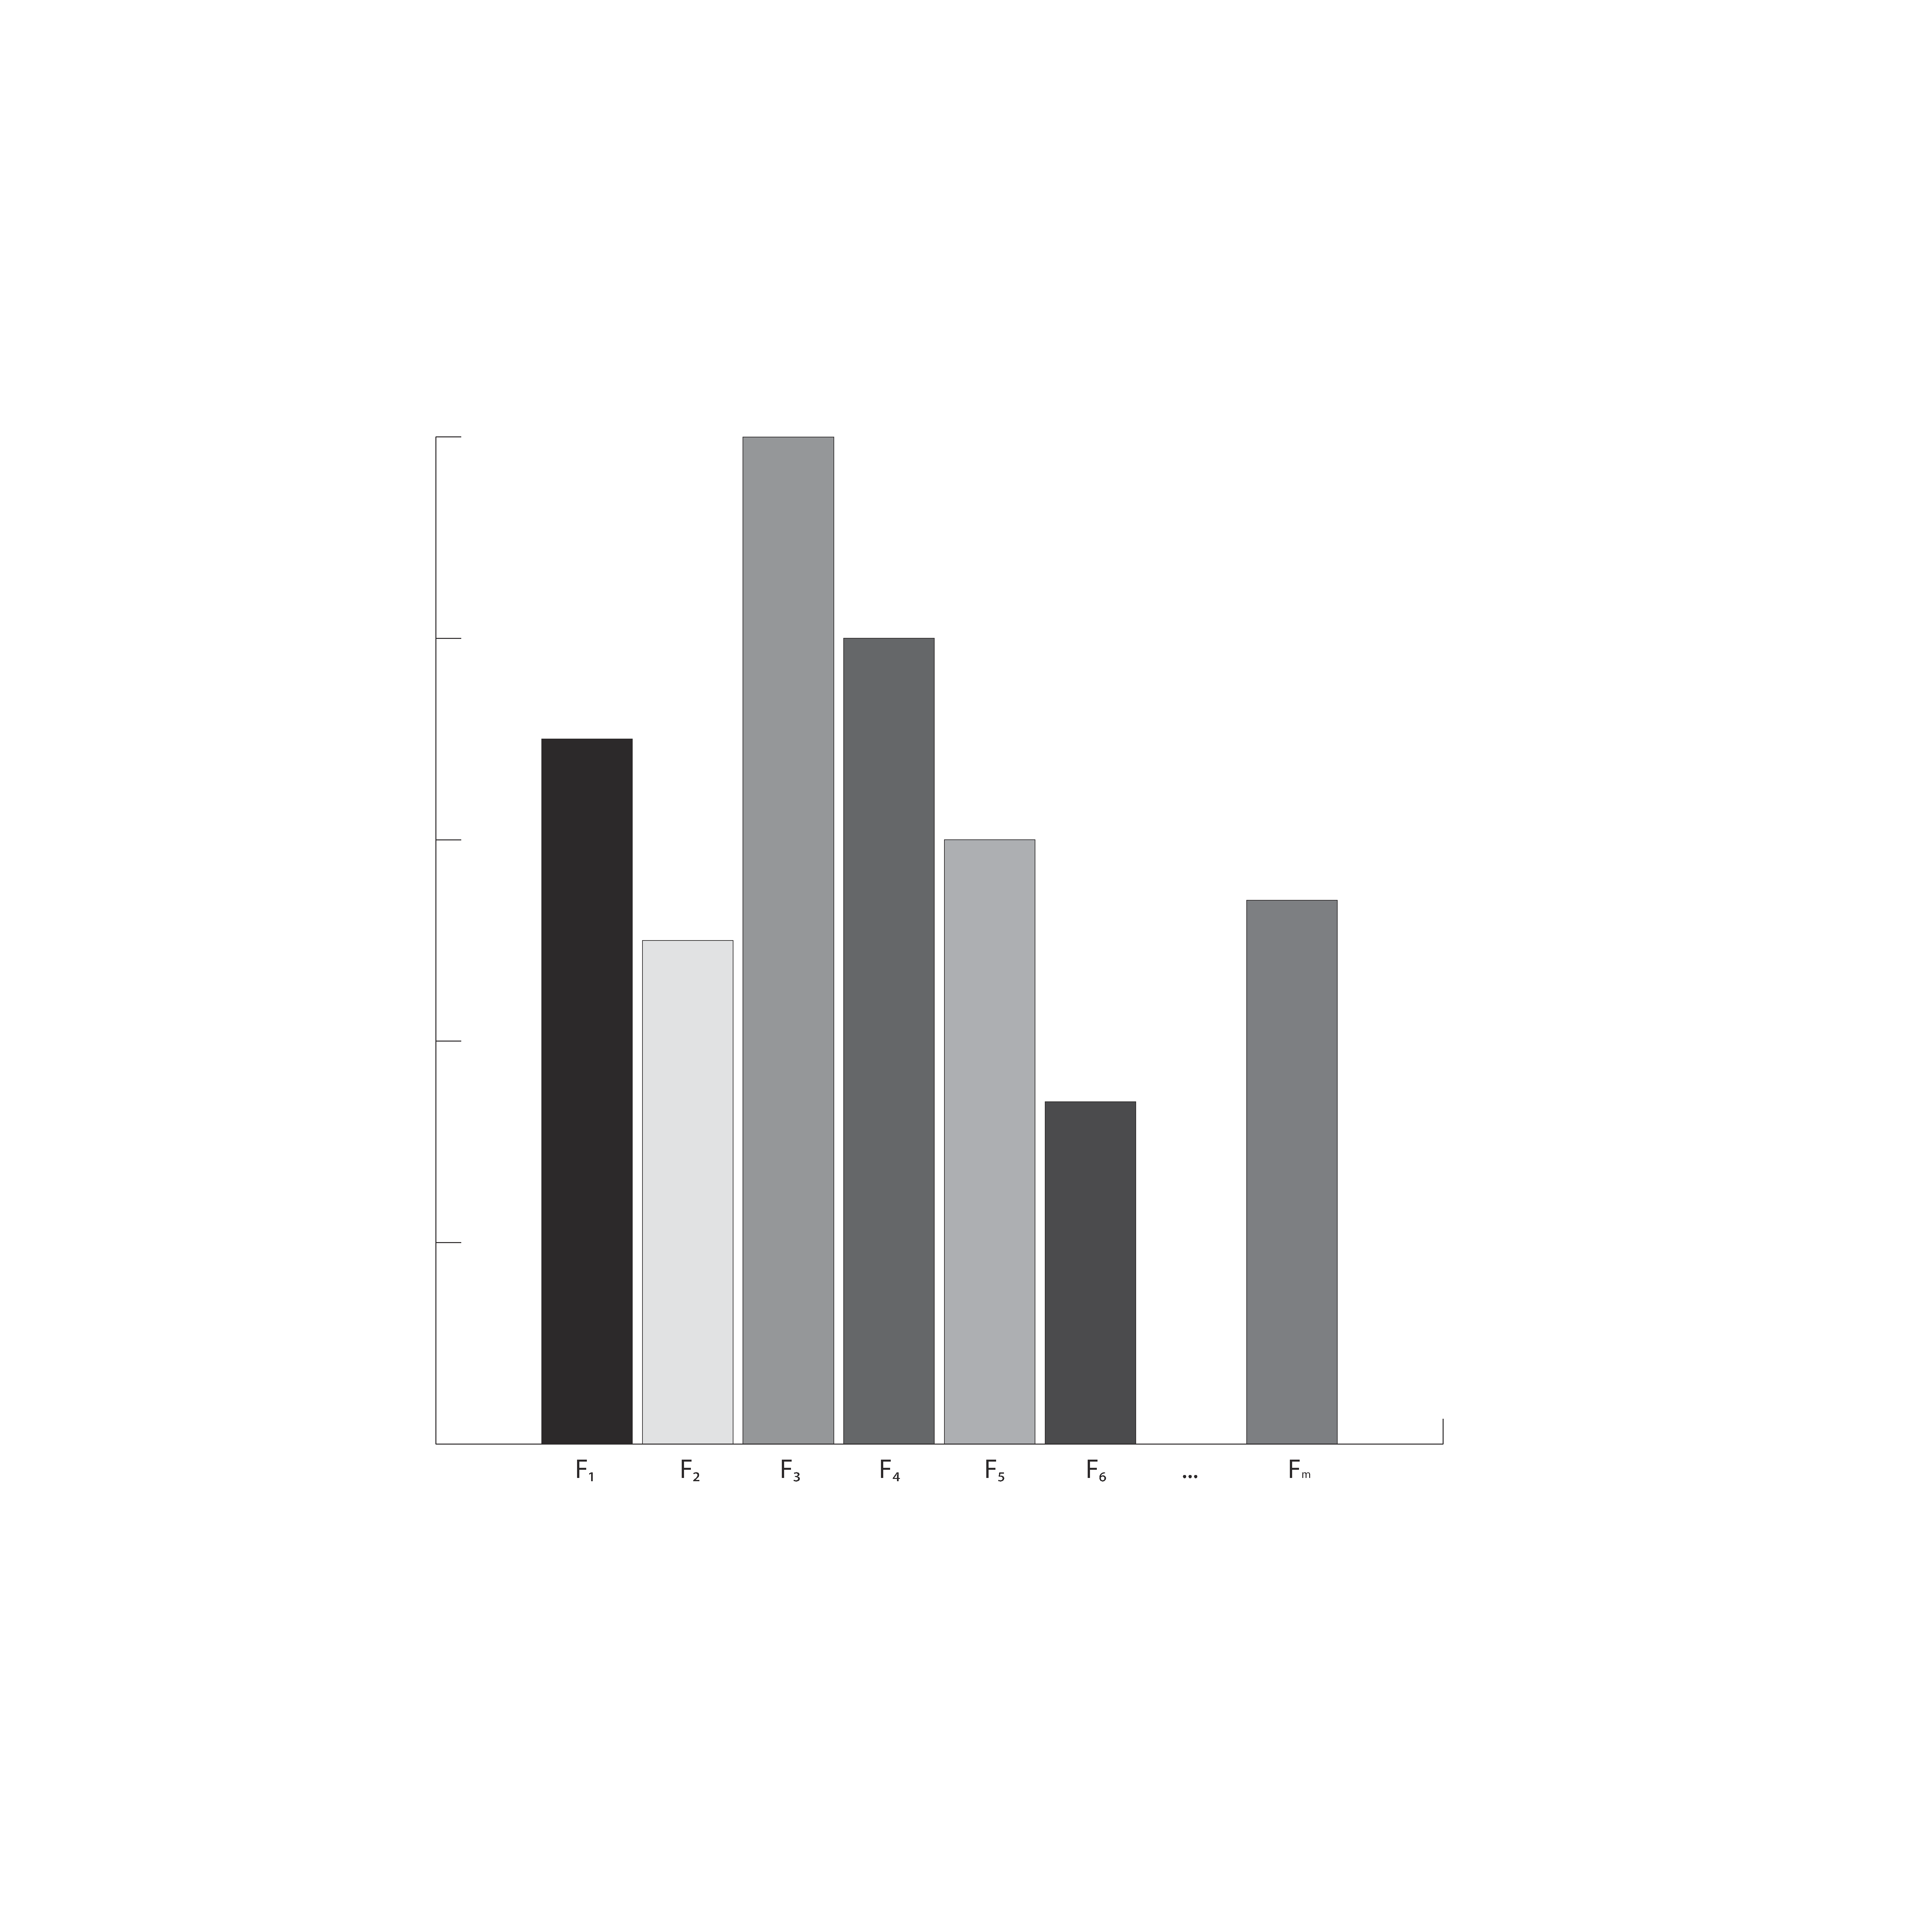
\includegraphics[width=\textwidth]{imagenes/marco_teorico/Descriptores_Fourier/Histograma_ejemplo_generico.pdf}
	\caption{}	
	\label{fig:fourier_histograma_generico_ejemplo}
\end{figure}

%% -----------------------------------------------------------------------%%

\section{Selección de características}

Una vez se han aplicado los métodos propuestos en la sección \ref{section:Extracción de catacterísticas}, es necesario realizar un análisis del poder clasificatorio de las características extraídas.

Para este trabajo, se han utilizado los siguientes métodos:
\begin{itemize}
	\item ANOVA
	\item SFS
\end{itemize}

\subsection{ANOVA}

\mynote{ANOVA es un conjunto de métodos estadísticos, entre los cuales está el F-Test, que es el que se usa aquí, principalmente.}

\mynote{Casi toda la información está sacada de \cite{frost_2020}.}

Conocido como Análisis de la Varianza (del inglés, \textit{ANalysis Of VAriance}).

Dado un ejemplo como una distribución de datos de dos clases (véase figura \ref{ANOVA:distribucion_ejemplo}), se disponen de dos características de clasificación: $(x,y)$.

\begin{figure}[h]
	\centering
	\captionsetup{justification=centering}
	\includegraphics[scale = 0.5]{imagenes/marco_teorico/ANOVA/ejemplo_distribuciones.png}
	\caption{Distribuciones para un caso ejemplo de ANOVA}
	\label{ANOVA:distribucion_ejemplo}
\end{figure}

La característica $x$ es mucho mejor que la $y$ a simple vista pues, comparando las distribuciones de ambas, para $x$ se obtienen dos distribuciones claramente separadas por completo, mientras que para la característica $y$ las distribuciones se solapan.

También se puede comprobar que la distribución para la característica $x$ presenta una menor varianza (son más compactas) que con $y$.

Por tanto, para este ejemplo se puede definir la condición \ref{eqn:anova_1} como un parámetro de discriminación de características. Cuanto mayor sea para una característica, mejor será su poder de clasificación.

\begin{equation}
	F = \dfrac{Distancia\:entre\:clases}{Compacidad\:de\:clases}
	\label{eqn:anova_1}
\end{equation}

Matemáticamente, la fórmula \ref{eqn:anova_1} puede expresarse de la siguiente forma siguiendo el método ANOVA:

\begin{itemize}
	\item El numerador (distancia entre clases) es definible con:
	\begin{equation}
		n_{azul}(\overline{x_{azul}}-\overline{x})^{2} + n_{rojo}(\overline{x_{rojo}}-\overline{x})^{2}
	\end{equation}
	\item El denominador (compacidad de clases), que no es sino la varianza de clases, puede expresarse como:
	\begin{equation}
		\left(\dfrac{1}{(n_{azul}-1)+(n_{roja}-1)}\right)\left(\sum_{i=1}^{n_{azul}}\left(x_{i}-\overline{x_{azul}}\right)^{2}+\sum_{i=1}^{n_{roja}}\left(x_{i}-\overline{x_{roja}}\right)^{2}\right)
	\end{equation}
\end{itemize}

De tal forma, la ecuación \ref{eqn:anova_1} queda como:

\begin{equation}
	F = \dfrac{n_{azul}(\overline{x_{azul}}-\overline{x})^{2} + n_{rojo}(\overline{x_{rojo}}-\overline{x})^{2}}{\left(\dfrac{1}{(n_{azul}-1)+(n_{roja}-1)}\right)\left(\sum_{i=1}^{n_{azul}}\left(x_{i}-\overline{x_{azul}}\right)^{2}+\sum_{i=1}^{n_{roja}}\left(x_{i}-\overline{x_{roja}}\right)^{2}\right)}
	\label{eqn:ANOVA}
\end{equation}

La ecuación \ref{eqn:ANOVA} da un parámetro para una variable (en este caso $x$). En un problema con $k$ características, se obtendrían $k$ valores de $F$, es decir, una $F$ para cada variable.

Utilizando las $k$ características extraídas con los métodos propuestos en \ref{section:Extracción de catacterísticas}, ANOVA proporcionaría $F_{k}$ valores, de entre los cuales se seleccionarían los $N$ con mayor valor $F$. La ecuación \ref{eqn:ANOVA_F} define el valor de F para un caso con $j = 1,\:2,\:3,\:...,\:N$ clases. 

\begin{equation}
	F = \dfrac{\sum_{j=1}^{N} n_{j}\left(\overline{x_{i}}-\overline{x}\right)^{2}}{\left(\dfrac{1}{\sum_{j=1}^{N}(n_{j}-1)}\right) \left(\sum_{j=1}^{N}\left(\sum_{i=1}^{n_{j}}(x_{i}-\overline{x_{j}})^{2}\right)\right)}
	\label{eqn:ANOVA_F}
\end{equation}

\mynote{Este método solo da información sobre lo bien que UNA variable discrimina, pero no dice como de bien lo harían varias juntas.}

\subsection{SFS}

Los algoritmos SFS (del inglés \textit{Sequential Feature Selector} son un conjunto de técnicas de selección de caracteríticas (algoritmos voraces) usados para reducir un espacio incial n-dimensional de características a otro k-dimensional donde $k\leq d$.

Si se tiene el siguiente conjunto n-dimensional $Y = \{y_{1},y_{2},y_{3},...,y_{n}\}$ de características de entrada, utilizando un estimador determinado (SVM, Knn, SDG, etc.) y una métrica de rendimiento determinada, el algoritmo SFS busca obtener un conjunto de salida $X_{k} = \{x_{j} | j = 1,2,...,d;\: x_{j}\epsilon Y\},\: con \:k = (0,1,2,...,n)$ tal que $X_{k}$ esté formado por las $k$ características que maximicen la métrica.

Existen dos formas de realizar este proceso: hacia adelante (\textit{Forward}) y hacia detrás (\textit{Backwards}).

\begin{itemize}
	\item Sequential Forward Selection: se comienza con un conjunto vacío $X_{0} = \emptyset / k = 0$. En cada iteración se aumenta el número de características hasta encontrar la combinación que de el mejor resultado (según la métrica a resolver).
	\item Sequential Backward Selection: se comienza con el conjunto inicial $Y$. En cada iteración se disminuye el número de características hasta encontrar la combinación que de el mejor resultado (según la métrica a resolver).
\end{itemize}

Es posible no llegar al mismo resultado empleando sentidos contrarios y tampoco obtener el mismo resultado, en varias iteraciones, utilizando el mismo método.

\mynote{En \textit{Sklearn} la métrica para su modelo SFS es una evaluación de validación cruzada con un estimador definido en la llamada al método SFS.}

\newpage
\section{Métodos de evalución}

Antes de entrar en la sección de modelos de clasificación, es necesario definir las métricas propuestas utilizadas para analizar los resultados de los clasificadores.

En una primera instancia, es necesario presentar la \nameref{tab:matriz_confusion}.

\begin{table}[h]
	\centering
	\caption{Matriz de confusión}
	\label{tab:matriz_confusion}
	\begin{tabular}{cc|cc|}
		\cline{3-4}
		&  & \multicolumn{2}{c|}{Valor real} \\ \cline{3-4} 
		&  & \multicolumn{1}{c|}{1}    & 0   \\ \hline
		\multicolumn{1}{|c|}{Valor}    & 1 & \multicolumn{1}{c|}{True Positive (TP)}  & False Positive (FP) \\ \cline{2-4} 
		\multicolumn{1}{|c|}{predicho} & 0 & \multicolumn{1}{c|}{False Negative (FN)} & True Negative (TN)  \\ \hline
	\end{tabular}
\end{table}

La matriz de confusión es una herramienta muy utilizada para representar y ver de forma sencilla los resultados de una clasificación. En el caso de la tabla \ref{tab:matriz_confusion}, se representa una matriz de confusión para un caso de clasificación binaria, sin embargo puede utilizarse para casos multiclases.


\subsubsection{Curva ROC}

Lo habitual, además de deseable, a la hora de obtener los valores predichos de un clasificador, es hacerlo en forma de estimaciones probabilísticas en el rango $[0,\:1]$. De tal forma que, cuando se obtenga un valor, se puede comprobar con qué nivel de confianza el clasificador asigna a qué clase la muestra a predecir.

Muchas librerías de algoritormos supervisados devuelven los resultados, por defecto, como valores enteros $0$ o $1$, aplicando un umbral de clasificación de $0.5$. En el caso de obtener $0.5000001$ para la clase positiva y $0.4999999$ para la negativa, el clasificador asignaría automáticamente la muestra a la clase positiva, obviando el hecho de que realmente no existe un nivel de confianza suficiente para clasificar la muestra de tal forma.

Al obtenerse probabilidades y no valores discretos, para asignar clases, es necesario establecer un umbral de clasificación por el cual si $p(n) \geq umbral \rightarrow n = 1$. Por tanto, es conveniente encontrar un valor para el umbral de clasificación que haga que el clasificador funcione lo mejor posible.

Para cada valor de umbral se obtiene una matriz de confusión diferente, así como sus pertinentes métricas. Puede que exista un valor de umbral en el que el clasificador, para la base de datos dada, sea idóneo o puede que no existe ningún valor de umbral que haga que el clasificador discrimine correctamente. Sin embargo, es posible que, independientemente del umbral, el clasificador obtenga buenos resultados.

Para poder analizar estos casos, se recurre a la curva ROC (del inglés \textit{Receiver operating characteristic}).

La curva ROC es un gráfico utilizado para determinar la abilidad discriminante de un clasificador binario según su umbral de clasificación es variado.

Este gráfico se basa en el espacio ROC, que es básicamente la representación de la tasa de verdaderos positivos (o exhaustividad) (\ref{eqn:exhaustividad}) frente a la tasa de falsos positivos (\ref{eqn:fpr}).

\mynote{Exhaustividad: cantidad de valores reales positivos predichos como positivos.}

\begin{equation}
	Exhaustividad\:(TPR) = \dfrac{TP}{P} = \dfrac{TP}{TP+FN}
	\label{eqn:exhaustividad}
\end{equation}

\begin{equation}
	Tasa\: de\: falsos\: positivos\:(FPR) = \dfrac{FP}{N} = \dfrac{FP}{FP+TN}
	\label{eqn:fpr}
\end{equation}

\begin{figure}[h]
	\centering
	\captionsetup{justification=centering}
	\includegraphics[width=0.5\textheight]{imagenes/marco_teorico/ROC/ROC_wiki.png}	
	\caption{Sacado de wikipedia (EDITAR)}
	\label{fig:roc_curva}
\end{figure}

La línea de puntos roja representa un clasificador puramente aleatorio que asigna un $0.5$ de probabilidades de pertencer a la clase positiva a cada muestra.

Para valores de umbral en el rango $[0,\:1]$, se obtienen los valores de \ref{eqn:exhaustividad} y \ref{eqn:fpr}, y se representa el punto correspondiente en el gráfico. De tal forma, se obtiene una curva escalonada que representa la calidad del clasificador.

El caso idóneo es aquel en el que la curva del clasificador es un escalón unidad, es decir, aquel clasificador que, para cualquier valor de umbral, se obtiene un 100\% de exhaustividad. Númericamente, este tipo de curva corresponde a una curva con una área bajo la curva de la unidad.

El peor caso es el clasificador cuya curva sea la inversa al escalón unidad pues, se obtiene un 0\% de exhaustividad para cualquier umbral, es decir, aquella curva con una área bajo la curva nula.

Por tanto, se define el parámetro \textbf{AUC}, del inglés \textit{Area Under the Curve}, que determina la calidad discriminante del clasificador. Cuanto mayor sea el valor de AUC, mejor el clasificador.

Sin embargo, la curva ROC no es correcta para casos desbalanceados ya que no representa correctamente los resultados, siendo necesario sustituirla por una curva de precisión-exhaustividad, que si lo hace \cite{10.1371/journal.pone.0118432}.

%\subsubsection{Métricas de rendimiento}
%
%A partir de la matriz de confusión se obtienen las llamadas métricas de rendimiento. Estos parámetros son utilizados en sistemas de clasificación, reconocimiento de patrones, etc, para analizar los resultados de dichos modelos.
%
%%\begin{itemize}
%%	\item Sensitividad, exhaustividad, tasa de positivos verdaderos: cantidad de valores reales positivos predichos como positivos.
%%		\begin{equation}
%%			Exhaustividad = \dfrac{TP}{P} = \dfrac{TP}{TP+FN}
%%			\label{eqn:exhaustividad}
%%		\end{equation}
%%	\item Exactitud: cantidad de predicciones que el modelo acertó.
%%		\begin{equation}
%%			Exactitud = \dfrac{TP+TN}{P+N} = \dfrac{TP+TN}{TP+TN+FP+FN}
%%			\label{eqn:exactitud}
%%		\end{equation}
%%	\item Precisión: cantidad de predicciones positivas acertadas correctamente.
%%		\begin{equation}
%%			Precision = \dfrac{TP}{TP+FP}
%%			\label{eqn:precision}
%%		\end{equation}
%%\end{itemize}
%
%Como se presenta en \cite{10.1371/journal.pone.0118432}, no todas las métricas de rendimiento son correctas para cualquier caso de clasificación, viéndose afectadas para casos desbalanceados.
%
%\mynote{Un caso desbalacenado de clasificación, binario o multiclase, es aquel donde la frecuencia de muestras de cada clase no es similar al del resto de clases. Es decir, para un caso binario, lo más común es tener muchas más muestras de la clase negativa (0) que de la positiva (1).}
%
%La imagen \ref{fig:comparacion_metricas} presenta la diferencia entre métricas para un caso desbalanceado respecto a un balanceado.
%
%\begin{figure}[h]
%	\centering
%	\captionsetup{justification=centering}
%	\includegraphics{imagenes/marco_teorico/Metricas/Tabla_articulo.png}
%	\caption{Métricas para caso balanceado y caso desbalanceado \cite{10.1371/journal.pone.0118432}}
%	\label{fig:comparacion_metricas}
%\end{figure}
%
%Muchas de las métricas mas usadas, como exactitud, tasa de falsos positivos o el error, no muestran diferencias entre casos.
%
%
%
